\documentclass[12pt]{article}
\usepackage{graphicx}
\usepackage{parskip}
\usepackage{url}
\usepackage{float}
\usepackage{setspace}
\graphicspath{ {./images/} }
\onehalfspacing

\begin{document}
\setlength{\parskip}{0pt}
\section*{Motor control}
In order to control the speed of the motors, one of
the potential options would be to use an H-bridge to control
the DC motors. However, that seemed unecessary, as another 
lighter and less power-consuming option would be to one 
N-channel mosfet for each motor.

\begin{figure}[H]
    \begin{center}
    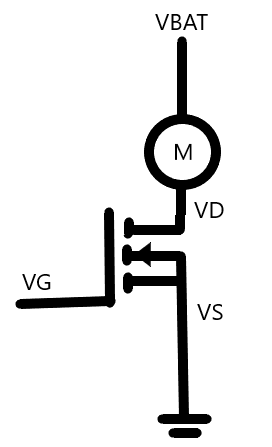
\includegraphics[scale=0.7]{Mosfet_Control}
    \end{center}
    \caption{Motor control with MOSFET.}
    \label{fig:Mosfet_Control}
\end{figure}

As illustrated in figure \ref{fig:Mosfet_Control}, the drain
of the MOSFET is connected to the Motor, which is supplied by 
the battery and the source of the MOSFET is grounded. 
Meanwhile, the VG pins are connected to one of the PWM pins 
of the nRF52840 MCU, where the opening of the gate is 
proportional to the PWM. Thus, when VG (simulated by PWM) is 
smaller than the V threshold of the MOSFET, the motors are 
static, and if VG surpasses V threshold, then the motors 
start spinning with higher RPM as PWM is increased. 
The MOSFETs used for this situation are FDD8896 \cite{FDD8896}, as it has 
a low threshold voltage of 2.5V (MCU pins can supply 
up to 3.3V), and can handle up 94A in continuous drain 
current.

\section*{MCU Overcurrent Protection}
In the process of building a quadcopter drone, one 
of the things needed to be configured was protection 
against overcurrent being drawn from the 
microcontroller. When the motors are switched on or off, 
a surge current arises which can result in additional 
overcurrent being pulled from the microcontroller if 
the battery is not alone capable of supplying the current. 

\begin{figure}[H]
    \begin{center}
    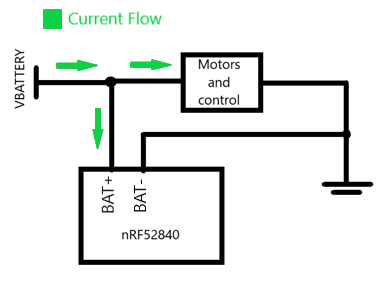
\includegraphics[scale=0.7]{Continuous_Current}
    \end{center}
    \caption{Current flow during continuous operation.}
    \label{fig:Continuous_Current}
\end{figure}

\begin{figure}[H]
    \begin{center}
    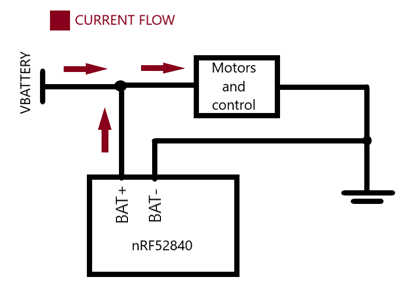
\includegraphics[scale=0.7]{Surge_Current}
    \end{center}
    \caption{Potential current flow due to surge current.}
    \label{fig:Surge_Current}
\end{figure}

In order to prevent reverse current from the MCU, 
during a surge, one of the potential options to 
utilise would be a diode placed in the following 
configuration. 

\begin{figure}[H]
    \begin{center}
    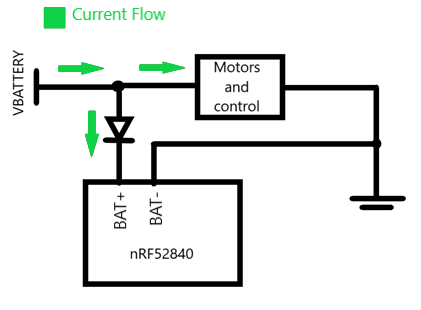
\includegraphics[scale=0.7]{Diode_Protection}
    \end{center}
    \caption{Diode added to prevent reverse current flow from MCU.}
    \label{fig:Diode_Protection}
\end{figure}

Additionally decoupling capacitors were added in 
parallel to the positive and negative motor pins 
and the MCU BAT+ and BAT- pins.


\begin{figure}[H]
    \begin{center}
    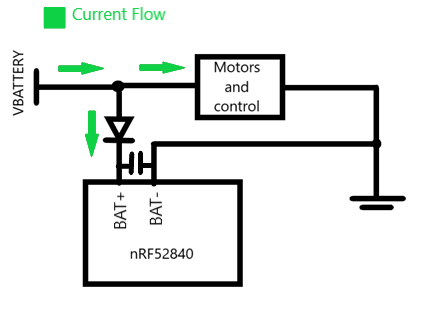
\includegraphics[scale=0.7]{Diode_Protection_&_decoupling_capacitors}
    \end{center}
    \caption{Example of decoupling capacitor for stable voltage to MCU.}
    \label{fig:Diode_Protection_&_decoupling_capacitors}
\end{figure}

The diode utilised is 1N5818 \cite{1N5818}, as it has a low 
forward voltage of under 0.5V, resulting in low 
power losses. Moreover, the decoupling capacitors
are cermaic capacitors as they generally smaller
in size, and they are rated at 100 nF, which follows 
the general guidelines of decoupling capacitor values.
\cite{DecouplingCap}

\bibliographystyle{plain}
\bibliography{Sources}

\end{document}
